\documentclass[12pt, letterpaper]{article}
\usepackage{graphicx} % Required for inserting images
\usepackage{hyperref}
\usepackage{listings}
\usepackage{amssymb}
\usepackage{amsmath}
\usepackage[english]{babel}
\usepackage{nicefrac, xfrac}
\usepackage{mathtools}
\newcommand{\acc}{\\\hphantom{}\\}
\usepackage[table,xcdraw]{xcolor}
\usepackage[paper=a4paper,left=20mm,right=20mm,bottom=25mm,top=25mm]{geometry}
\renewcommand{\labelenumii}{\arabic{enumi}.\arabic{enumii}}
\renewcommand{\labelenumiii}{\arabic{enumi}.\arabic{enumii}.\arabic{enumiii}}
\renewcommand{\labelenumiv}{\arabic{enumi}.\arabic{enumii}.\arabic{enumiii}.\arabic{enumiv}}
\title{\textbf{Travel to the moon}}

\date{}


\begin{document}

\maketitle


\section{Requisiti}
I dati di interesse per il sistema sono \acc
1. Requisiti sulle \textbf{crociere}:\\
\hphantom{ident}1.1. codice \\
\hphantom{ident}1.2. data di inizio\\
\hphantom{ident}1.3. data di fine\\
\hphantom{ident}1.4. nave utilizzata (v. req. 2)\\
\hphantom{ident}1.5. itinerario (v. req. 4)\\
\hphantom{ident}1.6. il tipo, uno tra:\\
\hphantom{ident}\hphantom{ident}1.6.1. luna di miele, di cui interessa:\\
\hphantom{ident}\hphantom{ident}\hphantom{ident}1.6.1.1. sottotipo, uno tra:\\
\hphantom{ident}\hphantom{ident}\hphantom{ident}\hphantom{ident}1.6.1.1.1. tradizionali\\
\hphantom{ident}\hphantom{ident}\hphantom{ident}\hphantom{ident}1.6.1.1.2. alternative\\
\hphantom{ident}\hphantom{ident}\hphantom{ident}1.6.2. per famiglie, di cui interessa:\\
\hphantom{ident}\hphantom{ident}\hphantom{ident}\hphantom{ident}1.6.3. se adatte ai bambini (booleano)
\acc
2. Requisiti sulle \textbf{navi}:\\
\hphantom{ident}2.1. nome\\
\hphantom{ident}2.2. comfort (3..5)\\
\hphantom{ident}2.3. capienza\acc
3. Requisiti sulle \textbf{destinazioni}:\\
\hphantom{ident}3.1. nome\\
\hphantom{ident}3.2. continente\\
\hphantom{ident}3.3. posti da vedere (v. req. 5)\\
\hphantom{ident}3.4. tipo, almeno uno tra:\\
\hphantom{ident}\hphantom{ident}3.4.1. romantico\\
\hphantom{ident}\hphantom{ident}3.4.2. divertente
\acc
4. Requisiti sugli \textbf{itinerari}:\\
\hphantom{ident}4.1. sequenza ordinata di elementi, di cui interessa:\\
\hphantom{ident}\hphantom{ident}4.1.1. porto (v. req. 3)\\
\hphantom{ident}\hphantom{ident}4.1.2. arrivo:\\
\hphantom{ident}\hphantom{ident}\hphantom{ident}4.1.2.1. il numero d'ordine del giorno (rispetto alla data di inizio della crociera)\\
\hphantom{ident}\hphantom{ident}\hphantom{ident}4.1.2.2. ora\\
\hphantom{ident}\hphantom{ident}4.1.3. ripartenza	\\
\hphantom{ident}\hphantom{ident}\hphantom{ident}4.1.3.1. il numero d'ordine del giorno (rispetto alla data di inizio della crociera)\\
\hphantom{ident}\hphantom{ident}\hphantom{ident}4.1.3.2. ora
\acc
5. Requisiti sui \textbf{posti da vedere}:\\
\hphantom{ident}5.1. nome\\
\hphantom{ident}5.2. descrizione\\
\hphantom{ident}5.3. orari di apertura, nella forma di una mappa che associa ad ogni giorno della settimana\\
\hphantom{ident}\hphantom{ident}(lunedì, ..., domenica) un insieme di fasce orarie, dove ogni fascia oraria\\
\hphantom{ident}\hphantom{ident}è definita in termini di una coppia di orari

\newpage
\section{Documenti di Specifica}
\subsection{Tipi di Dato}
TipoDestinazione = \{romantica, divertente\}\acc 
SottoTipo = \{tradizionale, alternativa\}\acc 
FasciaOraria = \{apertura : Time, chiusura : Time $>$ apertura\}

\newpage
\section{UML}\begin{center}
    
    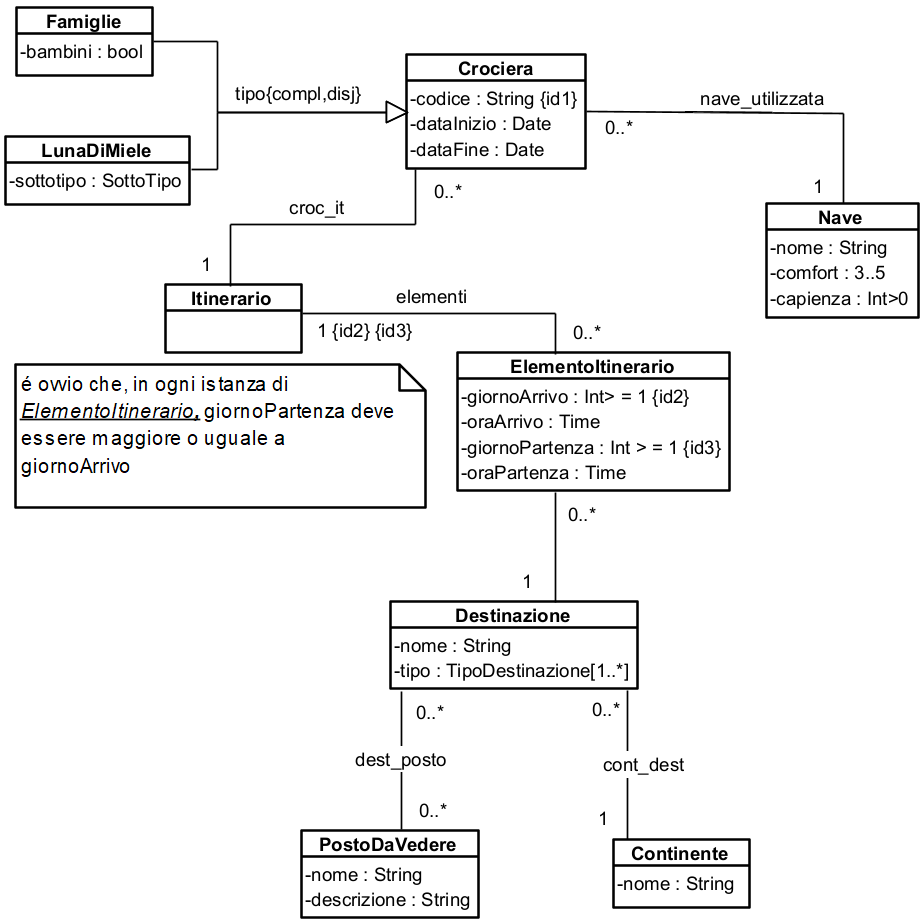
\includegraphics[width=\textwidth]{images/UML.png}
\end{center}


\end{document}

